%%%%%%%%%%%%%%%%%%%%%%%%%%%%%%%%%%%%%%%%%%%%%%%%%%%%%%%%%%%%%%%%%%%%%%%%%%%%%%%%%%
\begin{frame}[fragile]\frametitle{}
\begin{center}
{\Large Deep Q Learning}
\end{center}
\end{frame}

%%%%%%%%%%%%%%%%%%%%%%%%%%%%%%%%%%%%%%%%%%%%%%%%%%%%%%%%%%%%%%%%%%%%%%%%%%%%%%%%%%
\begin{frame}[fragile]\frametitle{Problems with Q Learning}


\begin{itemize}
\item Q Learning is suitable for small states space, tabular methods
\item Inefficient for Large and continuous state space problems.
\item Not enough time, resources.
\item Deep Learning comes to rescue here.
\item Neural Networks can be Universal Function approximator. Can model continuous function as well.
\end{itemize}

{\tiny (Ref: Modern Reinforcement Learning: Deep Q Learning in PyTorch - Phil Tabor)}

\end{frame}

%%%%%%%%%%%%%%%%%%%%%%%%%%%%%%%%%%%%%%%%%%%%%%%%%%%%%%%%%%%%%%%%%%%%%%%%%%%%%%%%%%
\begin{frame}[fragile]\frametitle{Deep Learning}


\begin{itemize}
\item Can approximate any function-relationship
\item Being primarily Matrix Multiplications, can leverage GPUs
\item Each perceptron is linear combination of inputs times weights plus bias.
\item Non linearity is added to it via Activation functions like Relu and Sigmoid.
\end{itemize}

{\tiny (Ref: Modern Reinforcement Learning: Deep Q Learning in PyTorch - Phil Tabor)}

\begin{center}
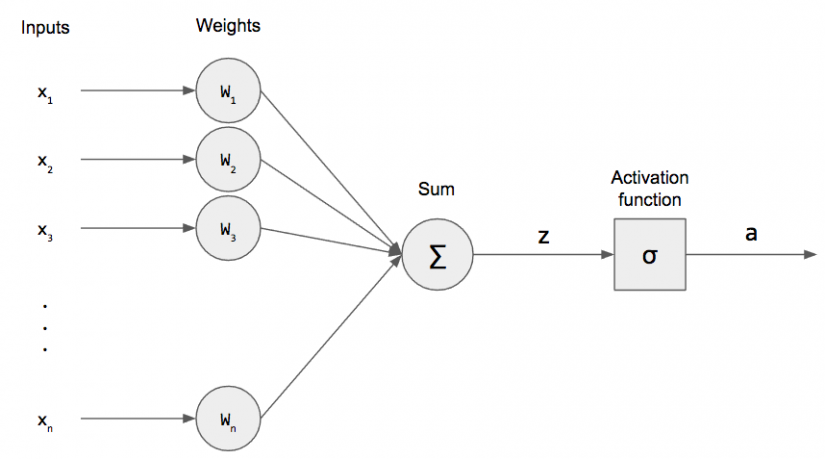
\includegraphics[width=0.6\linewidth,keepaspectratio]{rl69}

{\tiny (Ref: Python Machine Learning - Zenva)}
\end{center}

\end{frame}

%%%%%%%%%%%%%%%%%%%%%%%%%%%%%%%%%%%%%%%%%%%%%%%%%%%%%%%%%%%%%%%%%%%%%%%%%%%%%%%%%
\begin{frame}[fragile]\frametitle{Deep Learning Process}


\begin{itemize}
\item Input is fed into a layer and activated 
\item Result is then fed into next layer, and activated 
\item All the way through to the output
\item Output compared to some target to get cost 
\item  Weights changed to minimize cost (back propagation)
\item Repeat process $\rightarrow$ profit
\end{itemize}

{\tiny (Ref: Modern Reinforcement Learning: Deep Q Learning in PyTorch - Phil Tabor)}

\end{frame}

%%%%%%%%%%%%%%%%%%%%%%%%%%%%%%%%%%%%%%%%%%%%%%%%%%%%%%%%%%%%%%%%%%%%%%%%%%%%%%%%%
\begin{frame}[fragile]\frametitle{Deep Learning for Q Learning}


\begin{itemize}
\item Almost same structure as any standard but with MSE loss, Relu activation and a state-action-reward based Cost function
\item Inputs: states
\item Labels: actions
\item How it was made a supervised like learning problem? when there is no prior labeled data?
\item Target is $r + \gamma max Q(s',a_{max})$
\end{itemize}

{\tiny (Ref: Modern Reinforcement Learning: Deep Q Learning in PyTorch - Phil Tabor)}

\end{frame}

%%%%%%%%%%%%%%%%%%%%%%%%%%%%%%%%%%%%%%%%%%%%%%%%%%%%%%%%%%%%%%%%%%%%%%%%%%%%%%%%%%
\begin{frame}[fragile]\frametitle{From Q-Learning to Deep Q-Learning}

\begin{itemize}
\item The problem is that Q-Learning is a tabular method. Aka, a problem in which the state and actions spaces are small enough to approximate value functions to be represented as arrays and tables. And this is not scalable. FrozenLake, we had 14 states. Taxi-v3, we had 500 states.
\item For large state spaces creating and updating a Q-table for that environment would not be efficient. In this case, the best idea is to approximate the Q-values instead of a Q-table using a parametrized Q-function $Q_{\theta}(s,a)$. Neural network will approximate, given a state, the different Q-values for each possible action at that state. And that's exactly what Deep Q-Learning does.
\end{itemize}


{\tiny (Ref: Chapter 3 of the Deep Reinforcement Learning Class with Hugging Face)}

\end{frame}

%%%%%%%%%%%%%%%%%%%%%%%%%%%%%%%%%%%%%%%%%%%%%%%%%%%%%%%%%%%%%%%%%%%%%%%%%%%%%%%%%%
\begin{frame}[fragile]\frametitle{The Deep Q-Network (DQN)}

\begin{center}
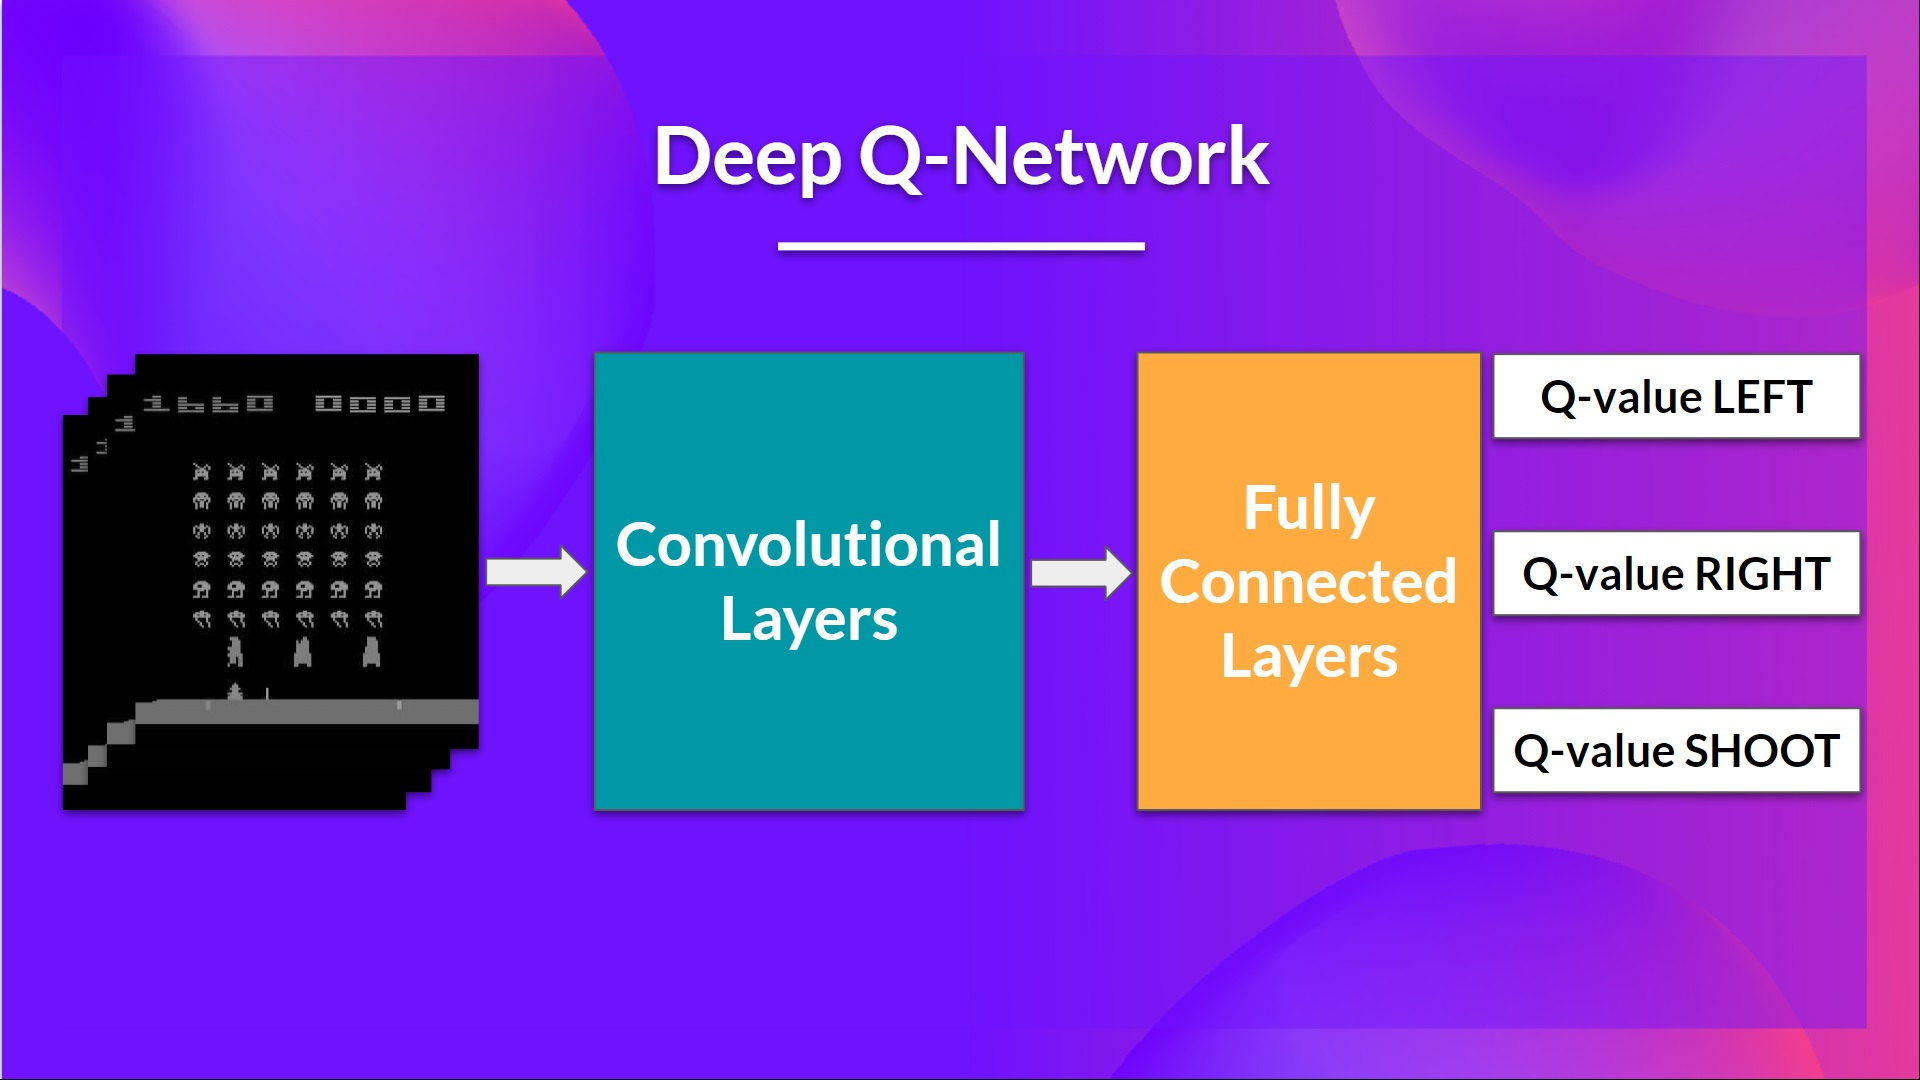
\includegraphics[width=0.5\linewidth,keepaspectratio]{rl106}
\end{center}

\begin{itemize}
\item As input, we take a stack of 4 frames passed through the network as a state and output a vector of Q-values for each possible action at that state. Then, like with Q-Learning, we just need to use our epsilon-greedy policy to select which action to take.

\item When the Neural Network is initialized, the Q-value estimation is terrible. But during training, our Deep Q-Network agent will associate a situation with appropriate action and learn to play the game well.
\end{itemize}

{\tiny (Ref: Chapter 3 of the Deep Reinforcement Learning Class with Hugging Face)}

\end{frame}

%%%%%%%%%%%%%%%%%%%%%%%%%%%%%%%%%%%%%%%%%%%%%%%%%%%%%%%%%%%%%%%%%%%%%%%%%%%%%%%%%%
\begin{frame}[fragile]\frametitle{The Deep Q-Learning Algorithm)}

\begin{center}
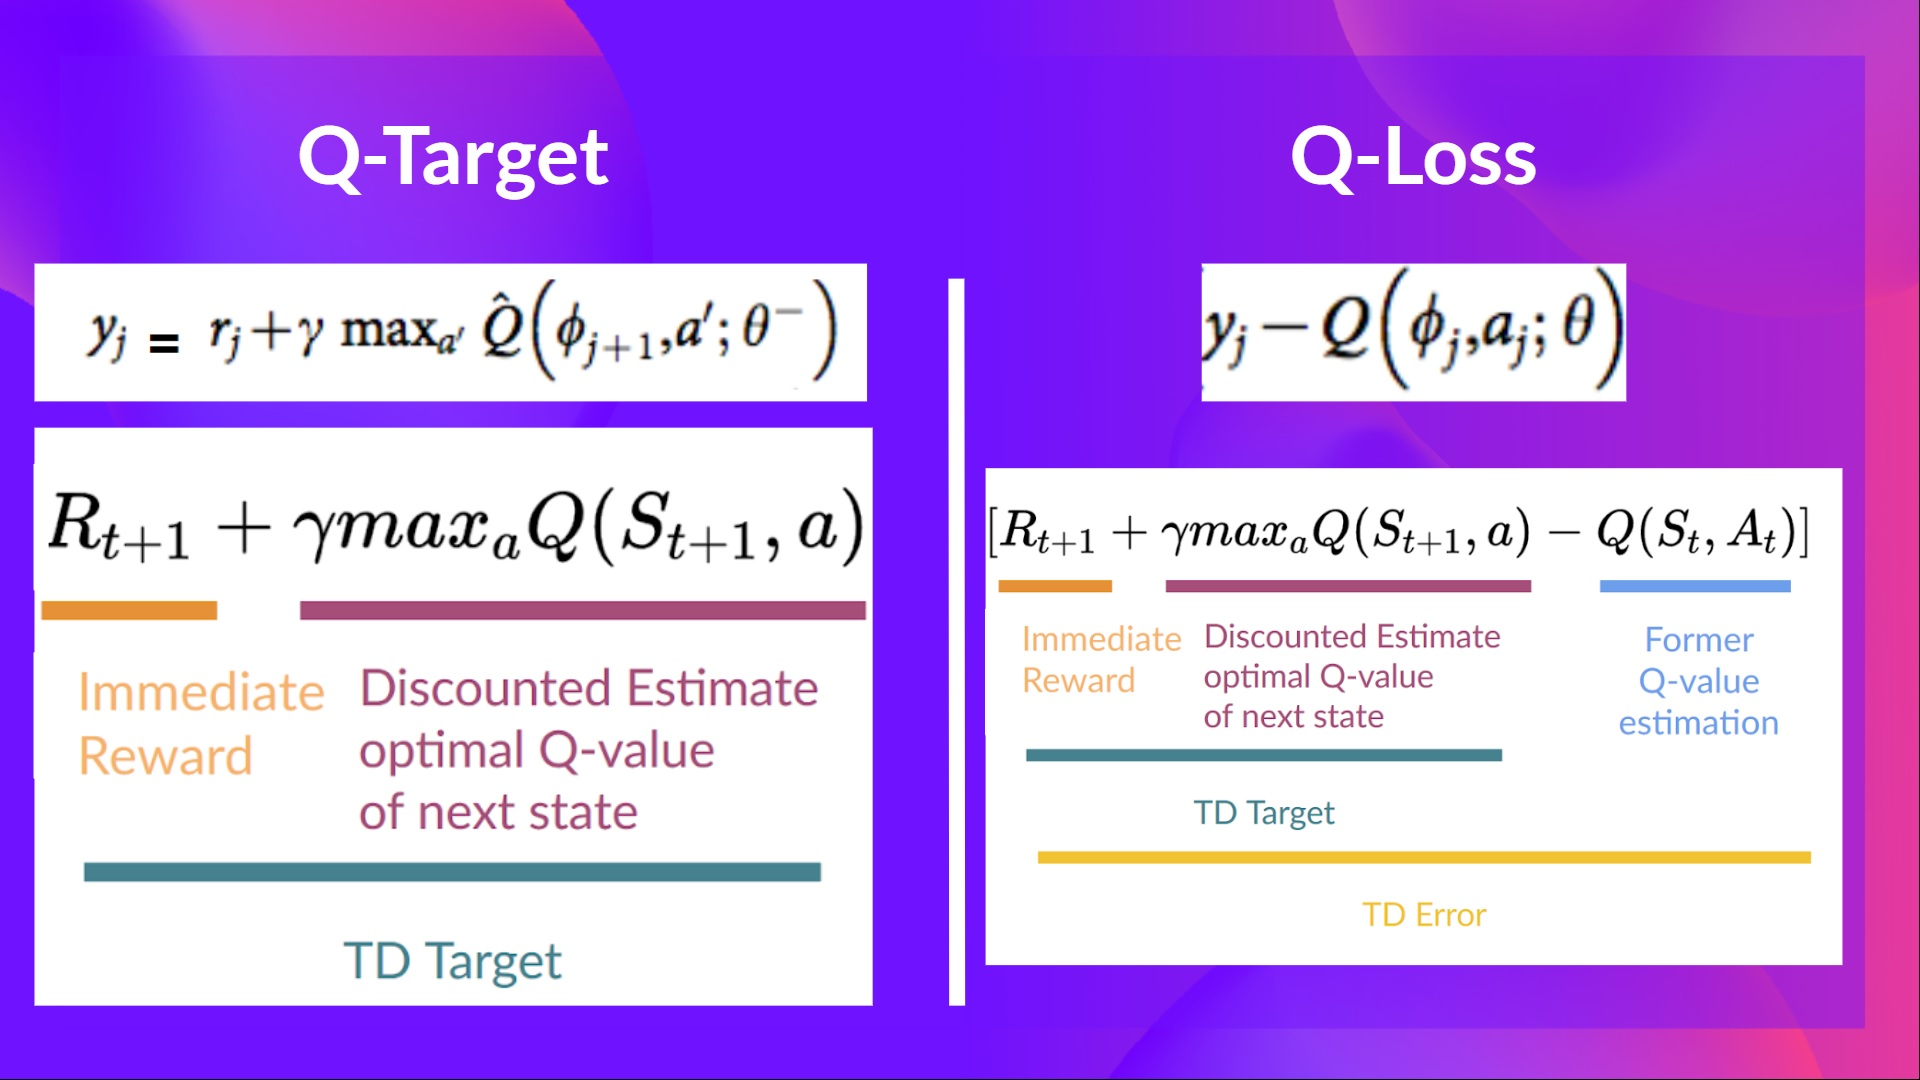
\includegraphics[width=0.8\linewidth,keepaspectratio]{rl107}
\end{center}

In Deep Q-Learning, we create a Loss function between our Q-value prediction and the Q-target and use Gradient Descent to update the weights of our Deep Q-Network to approximate our Q-values better.

{\tiny (Ref: Chapter 3 of the Deep Reinforcement Learning Class with Hugging Face)}

\end{frame}

%%%%%%%%%%%%%%%%%%%%%%%%%%%%%%%%%%%%%%%%%%%%%%%%%%%%%%%%%%%%%%%%%%%%%%%%%%%%%%%%%%
\begin{frame}[fragile]\frametitle{The Deep Q-Learning Algorithm)}

Two phases

\begin{itemize}
\item Sampling: we perform actions and store the observed experiences tuples in a replay memory.
\item Training: Select the small batch of tuple randomly and learn from it using a gradient descent update step.
\end{itemize}

But, this is not the only change compared with Q-Learning. Deep Q-Learning training might suffer from instability, mainly because of combining a non-linear Q-value function (Neural Network) and bootstrapping (when we update targets with existing estimates and not an actual complete return).

{\tiny (Ref: Chapter 3 of the Deep Reinforcement Learning Class with Hugging Face)}

\end{frame}

%%%%%%%%%%%%%%%%%%%%%%%%%%%%%%%%%%%%%%%%%%%%%%%%%%%%%%%%%%%%%%%%%%%%%%%%%%%%%%%%%%
\begin{frame}[fragile]\frametitle{The Deep Q-Learning Algorithm)}

To help us stabilize the training, we implement three different solutions:


\begin{itemize}
\item Experience Replay, to make more efficient use of experiences.
\item Fixed Q-Target to stabilize the training.
\item Double Deep Q-Learning, to handle the problem of the overestimation of Q-values.
\end{itemize}

{\tiny (Ref: Chapter 3 of the Deep Reinforcement Learning Class with Hugging Face)}

\end{frame}


%%%%%%%%%%%%%%%%%%%%%%%%%%%%%%%%%%%%%%%%%%%%%%%%%%%%%%%%%%%%%%%%%%%%%%%%%%%%%%%%%%
\begin{frame}[fragile]\frametitle{Experience Replay to make more efficient use of experiences}

Why do we create a replay memory?

Experience Replay in Deep Q-Learning has two functions:


\begin{itemize}
\item Make more efficient use of the experiences during the training
\item Experience replay helps us make more efficient use of the experiences during the training. Usually, in online reinforcement learning, we interact in the environment, get experiences (state, action, reward, and next state), learn from them (update the neural network) and discard them.
\item But with experience replay, we create a replay buffer that saves experience samples that we can reuse during the training.
\item This allows us to learn from individual experiences multiple times.
\item Avoid forgetting previous experiences and reduce the correlation between experiences
\end{itemize}


{\tiny (Ref: Chapter 3 of the Deep Reinforcement Learning Class with Hugging Face)}

\end{frame}

%%%%%%%%%%%%%%%%%%%%%%%%%%%%%%%%%%%%%%%%%%%%%%%%%%%%%%%%%%%%%%%%%%%%%%%%%%%%%%%%%%
\begin{frame}[fragile]\frametitle{Experience Replay to make more efficient use of experiences}


\begin{itemize}
\item The solution is to create a Replay Buffer that stores experience tuples while interacting with the environment and then sample a small batch of tuples. This prevents the network from only learning about what it has immediately done.
\item Experience replay also has other benefits. By randomly sampling the experiences, we remove correlation in the observation sequences and avoid action values from oscillating or diverging catastrophically.
\end{itemize}


{\tiny (Ref: Chapter 3 of the Deep Reinforcement Learning Class with Hugging Face)}

\end{frame}

%%%%%%%%%%%%%%%%%%%%%%%%%%%%%%%%%%%%%%%%%%%%%%%%%%%%%%%%%%%%%%%%%%%%%%%%%%%%%%%%%%
\begin{frame}[fragile]\frametitle{Fixed Q-Target to stabilize the training}


\begin{itemize}
\item When we want to calculate the TD error (aka the loss), we calculate the difference between the TD target (Q-Target) and the current Q-value (estimation of Q).
\item But we don’t have any idea of the real TD target. We need to estimate it. Using the Bellman equation, we saw that the TD target is just the reward of taking that action at that state plus the discounted highest Q value for the next state.
\item However, the problem is that we are using the same parameters (weights) for estimating the TD target and the Q value. Consequently, there is a significant correlation between the TD target and the parameters we are changing.
\item Therefore, it means that at every step of training, our Q values shift but also the target value shifts. So, we’re getting closer to our target, but the target is also moving. It’s like chasing a moving target! This led to a significant oscillation in training
\end{itemize}


{\tiny (Ref: Chapter 3 of the Deep Reinforcement Learning Class with Hugging Face)}

\end{frame}



%%%%%%%%%%%%%%%%%%%%%%%%%%%%%%%%%%%%%%%%%%%%%%%%%%%%%%%%%%%%%%%%%%%%%%%%%%%%%%%%%%
\begin{frame}[fragile]\frametitle{Double DQN}


\begin{itemize}
\item Double DQNs, or Double Learning, were introduced by Hado van Hasselt. 
\item Handles the problem of the overestimation of Q-values.
\item Remember: a simple problem while calculating the TD target: how are we sure that the best action for the next state is the action with the highest Q-value?
\item Accuracy of Q values depends on what action we tried and what neighboring states we explored.
\item Not enough information about the best action to take at the beginning of the training. Therefore, taking the maximum Q value (which is noisy) as the best action to take can lead to false positives. If non-optimal actions are regularly given a higher Q value than the optimal best action, the learning will be complicated.
\item Solution: to compute the Q target, use two networks to decouple the action selection from the target Q value generation. 
\item Use DQN network to select the best action to take for the next state (the action with the highest Q value).
\item Use Target network to calculate the target Q value of taking that action at the next state.
\end{itemize}

Double DQN helps train faster and have more stable learning.

{\tiny (Ref: Chapter 3 of the Deep Reinforcement Learning Class with Hugging Face)}

\end{frame}




%%%%%%%%%%%%%%%%%%%%%%%%%%%%%%%%%%%%%%%%%%%%%%%%%%%%%%%%%%%%%%%%%%%%%%%%%%%%%%%%%%
\begin{frame}[fragile]\frametitle{Deep RL Algorithms}

There are many different kinds of RL algorithms! This is a non-exhaustive taxonomy (with specific algorithms in blue):
\begin{figure}
\centering
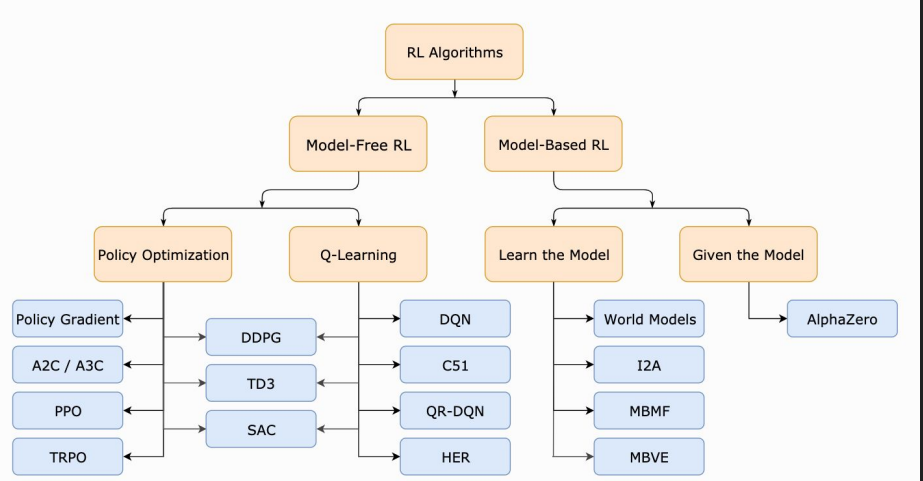
\includegraphics[width=\linewidth]{rl16}
\end{figure}

{\tiny (Ref: Intro to RL - Joshua Achiam)}


\end{frame}

%%%%%%%%%%%%%%%%%%%%%%%%%%%%%%%%%%%%%%%%%%%%%%%%%%%%%%%%%%%%%%%%%%%%%%%%%%%%%%%%%%
\begin{frame}[fragile]\frametitle{Deep RL Algorithms}

Using Model-Free RL Algorithms:
\begin{center}
\begin{tabular}{c|c|c}
Algorithm &  $a$ Discrete &$a$  Continuous \\ \hline
Policy optimization & Yes & Yes \\
DQN / C51 / QR-DQN & Yes & \color{red}{No} \\
DDPG & \color{red}{No} & Yes
\end{tabular}
\end{center}

Using Model-Based RL Algorithms:
\begin{itemize}
\item Learning the model means learning to generate next state and/or reward:
%
\begin{equation*}
\hat{s}_{t+1}, \hat{r}_t = \hat{f}_{\phi}(s_t, a_t)
\end{equation*}
\item Some algorithms may only work with an \textit{exact} model of the environment
\begin{itemize}
\item AlphaZero uses the rules of the game to build its search tree
\end{itemize}
\end{itemize}

{\tiny (Ref: Intro to RL - Joshua Achiam)}


\end{frame}

%%%%%%%%%%%%%%%%%%%%%%%%%%%%%%%%%%%%%%%%%%%%%%%%%%%%%%%%%%%%%%%%%%%%%%%%%%%%%%%%%%
\begin{frame}[fragile]\frametitle{Policy Gradients}

\begin{itemize}
\item An algorithm for training stochastic policies:
\begin{itemize}
\item Run current policy in the environment to collect rollouts
\item Take stochastic gradient ascent on policy performance using the \textbf{policy gradient}:
\begin{align*}
g &= \nabla_{\theta} E_{\tau \sim \pi_{\theta}}{\sum_{t=0}^T r_t} \\
&= E_{\tau \sim \pi_{\theta}}{\sum_{t=0}^T \nabla_{\theta} \log \pi_{\theta}(a_t | s_t) \left(\sum_{t'=t}^T r_{t'}\right)}\\
&\approx \frac{1}{|D|}\sum_{\tau \in D} \sum_{t=0}^T \nabla_{\theta} \log \pi_{\theta}(a_t | s_t) \left(\sum_{t'=t}^T r_{t'}\right)
\end{align*}
\end{itemize}
\item Core idea: up probabilities of good actions and down of bad actions
\item Sum of rewards after time $t$ is the \textit{reward-to-go} at time $t$: $\hat{R}_t = \sum_{t'=t}^T r_{t'}$
\end{itemize}

{\tiny (Ref: Intro to RL - Joshua Achiam)}


\end{frame}

%%%%%%%%%%%%%%%%%%%%%%%%%%%%%%%%%%%%%%%%%%%%%%%%%%%%%%%%%%%%%%%%%%%%%%%%%%%%%%%%%%
\begin{frame}[fragile]\frametitle{Example Implementation}

Make the model, loss function, and optimizer:
\begin{lstlisting}
 # make model
 with tf.variable_scope('model'):
     obs_ph = tf.placeholder(shape=(None, obs_dim), dtype=tf.float32)
     net = mlp(obs_ph, hidden_sizes=[hidden_dim]*n_layers)
     logits = tf.layers.dense(net, units=n_acts, activation=None)
     actions = tf.squeeze(tf.multinomial(logits=logits,num_samples=1), axis=1)

 # make loss
 adv_ph = tf.placeholder(shape=(None,), dtype=tf.float32)
 act_ph = tf.placeholder(shape=(None,), dtype=tf.int32)
 action_one_hots = tf.one_hot(act_ph, n_acts)
 log_probs = tf.reduce_sum(action_one_hots * tf.nn.log_softmax(logits), axis=1)
 loss = -tf.reduce_mean(adv_ph * log_probs)

 # make train op
 train_op = tf.train.AdamOptimizer(learning_rate=lr).minimize(loss)

 sess = tf.InteractiveSession()
 sess.run(tf.global_variables_initializer())
\end{lstlisting}


\end{frame}

%%%%%%%%%%%%%%%%%%%%%%%%%%%%%%%%%%%%%%%%%%%%%%%%%%%%%%%%%%%%%%%%%%%%%%%%%%%%%%%%%%
\begin{frame}[fragile]\frametitle{One iteration of training}
\begin{lstlisting}
# train model for one iteration
batch_obs, batch_acts, batch_rtgs, batch_rets, batch_lens = [], [], [], [], []
obs, rew, done, ep_rews = env.reset(), 0, False, []
while True:
    batch_obs.append(obs.copy())
    act = sess.run(actions, {obs_ph: obs.reshape(1,-1)})[0]
    obs, rew, done, _ = env.step(act)
    batch_acts.append(act)
    ep_rews.append(rew)
    if done:
        batch_rets.append(sum(ep_rews))
        batch_lens.append(len(ep_rews))
        batch_rtgs += list(discount_cumsum(ep_rews, gamma))
        obs, rew, done, ep_rews = env.reset(), 0, False, []
        if len(batch_obs) > batch_size:
            break
# normalize advs trick:
batch_advs = np.array(batch_rtgs)
batch_advs = (batch_advs - np.mean(batch_advs))/(np.std(batch_advs) + 1e-8)
batch_loss, _ = sess.run([loss,train_op], feed_dict={obs_ph: np.array(batch_obs),act_ph: np.array(batch_acts), adv_ph: batch_advs})
\end{lstlisting}


\end{frame}

%%%%%%%%%%%%%%%%%%%%%%%%%%%%%%%%%%%%%%%%%%%%%%%%%%%%%%%%%%%%%%%%%%%%%%%%%%%%%%%%%%
\begin{frame}[fragile]\frametitle{Getting Q-Learning to Work (DQN)}

Experience replay:
\begin{itemize}
\item Data distribution changes over time: as your $Q$ function gets better and you \textit{exploit} this, you visit different $(s,a,s',r)$ transitions than you did earlier
\item Stabilize learning by keeping old transitions in a replay buffer, and taking minibatch gradient descent on mix of old and new transitions
\end{itemize}
Target networks:
\begin{itemize}
\item Minimizing Bellman error directly is unstable! 
\item It's \textit{like} regression, but it's not:
%
\begin{equation*}
\min_{\theta} \sum_{(s,a,s',r)\in D} \left(Q_{\theta}(s,a) - y(s',r) \right)^2,
\end{equation*}
%
where the target $y(s',r)$ is
%
\begin{equation*}
y(s',r) = r + \gamma \max_{a'} Q_{\theta}(s',a').
\end{equation*}
%
Targets depend on parameters $\theta$---so an update to $Q$ changes the target!
\item Stabilize it by \textit{holding the target fixed} for a while: keep a separate target network, $Q_{\theta_{targ}}$, and every $k$ steps update $\theta_{targ} \leftarrow \theta$
\end{itemize}
{\tiny (Ref: Intro to RL - Joshua Achiam)}


\end{frame}

%%%%%%%%%%%%%%%%%%%%%%%%%%%%%%%%%%%%%%%%%%%%%%%%%%%%%%%%%%%%%%%%%%%%%%%%%%%%%%%%%%
\begin{frame}[fragile]\frametitle{DQN Pseudocode}

\begin{algorithm}[H]
\tiny
   \caption{Deep Q-Learning}
   \label{alg1}
\begin{algorithmic}
     \STATE Randomly generate $Q$-function parameters $\theta$
     \STATE Set target $Q$-network parameters $\theta_{targ} \leftarrow \theta$
     \STATE Make empty replay buffer $D$
	 \STATE Receive observation $s_0$ from environment
	 \FOR{$t = 0,1,2,...$} 
	 \STATE With probability $\epsilon$, select random action $a_t$; otherwise select $a_t = \arg \max_{a} Q_{\theta}(s_t, a)$
	 \STATE Step environment to get $s_{t+1}, r_t$ and end-of-episode signal $d_t$
	 \STATE Linearly decay $\epsilon$ until it reaches final value $\epsilon_f$
	 \STATE Store $(s_t, a_t, r_t, s_{t+1}, d_t) \to D$
	 \STATE Sample mini-batch of transitions $B = \{(s,a,r,s',d)_i\}$ from $ D$
	 \STATE For each transition in $B$, compute 
	 \begin{equation*}
	 y = \left\{ \begin{array}{ll}
	 r & \text{transition is terminal }(d=\text{True}) \\
	 r + \gamma \max_{a'} Q_{\theta_{targ}}(s', a') & \text{otherwise}
	 \end{array}\right.
	 \end{equation*}
	 \STATE Update $Q$ by gradient descent on regression loss:
	 \begin{equation*}
	 \theta \leftarrow \theta - \alpha \nabla_{\theta} \sum_{(s,a,y)\in B} \left(Q_{\theta}(s,a) - y \right)^2
	 \end{equation*}
	 \IF{ $t \% t_{update} =0$}
	 	\STATE Set $\theta_{targ} \leftarrow \theta$
	 \ENDIF
	\ENDFOR
\end{algorithmic}
\end{algorithm}

{\tiny (Ref: Intro to RL - Joshua Achiam)}


\end{frame}
